\documentclass[aps,prb,preprint,superscriptaddress,floatfix]{revtex4-2}
\usepackage[utf8]{inputenc}
\usepackage{graphicx}
\usepackage{amsmath,amssymb}
\usepackage{longtable}
\usepackage[colorlinks=true,linkcolor=blue,citecolor=blue,urlcolor=blue]{hyperref}
\graphicspath{{figures/}}
\renewcommand{\thefigure}{S\arabic{figure}}
\renewcommand{\thetable}{S\arabic{table}}
\renewcommand{\theequation}{S\arabic{equation}}
\renewcommand{\thesection}{S\arabic{section}}
\newcommand{\Tc}{$T_c$}

\begin{document}

\title{Supplemental Material for\\
``Compositional complexity does not raise $T_c$: an active-learning KKR-CPA search for bcc refractory high-entropy superconductors''}

\author{Author}
\affiliation{Affiliation 1}
\author{Author 2}
\affiliation{Affiliation 2}

\date{\today}
\maketitle

\tableofcontents

\clearpage
\section{Literature data used for validation}
\label{sec:literature}

Table~\ref{tab:lit} lists all published \Tc\ values used in Fig.~1 of the main text, in
order of decreasing measured \Tc. The composition is the nominal one of the source; where the
same composition was measured in several papers, each measurement is a separate entry.
Entries marked $^\dagger$ were reported as multiphase, or with an incomplete
characterisation, in the source. The calculated value is $T_c^{\rm corr}$ of the present
work, which equals $T_c(\mu^* = 0.1)$ for the alloys without V and Sc.

{\footnotesize
\begin{longtable}{@{}lccl@{\hspace{1.2em}}lccl@{}}
\caption{Literature bcc alloys: measured and calculated \Tc\ (K).}
\label{tab:lit}\\
\hline\hline
composition & $T_c^{\rm exp}$ & $T_c^{\rm calc}$ & ref. & composition & $T_c^{\rm exp}$ & $T_c^{\rm calc}$ & ref. \\
\hline
\endfirsthead
\hline
composition & $T_c^{\rm exp}$ & $T_c^{\rm calc}$ & ref. & composition & $T_c^{\rm exp}$ & $T_c^{\rm calc}$ & ref. \\
\hline
\endhead
\hline\hline
\endfoot
Nb$_{67}$Ti$_{11}$Zr$_{11}$Hf$_{11}$ & 9.36 & 13.31 & \cite{lit_vonRohr_15926113} & Nb$_{25}$Ta$_{25}$Hf$_{22}$Ti$_{20}$Sc$_{8}$$^{\dagger}$ & 6.60 & 5.62 & \cite{lit_Krnel_15031122} \\
Nb$_{90}$Ti$_{3}$Hf$_{3}$Ta$_{3}$ & 9.11 & 13.86 & \cite{lit_Li_ad9fa8} & Nb$_{30}$Ti$_{25}$Hf$_{25}$Sc$_{20}$$^{\dagger}$ & 6.60 & 5.24 & \cite{lit_Krnel_15031122} \\
Nb$_{75}$Ti$_{8}$Hf$_{8}$Ta$_{8}$ & 8.82 & 11.77 & \cite{lit_Li_ad9fa8} & Sc$_{20}$Ti$_{20}$Nb$_{20}$Hf$_{20}$Ta$_{20}$$^{\dagger}$ & 6.60 & 5.21 & \cite{lit_Krnel_15031122} \\
Nb$_{32}$Zr$_{26}$Ti$_{24}$Sc$_{18}$$^{\dagger}$ & 8.40 & 10.13 & \cite{lit_Krnel_15031122} & Nb$_{34}$Ta$_{34}$Ti$_{11}$Hf$_{11}$Sc$_{7}$Mo$_{4}$ & 6.60 & 7.03 & \cite{lit_vonRohr_s2034801} \\
Sc$_{25}$Ti$_{25}$Zr$_{25}$Nb$_{25}$$^{\dagger}$ & 8.40 & 9.55 & \cite{lit_Krnel_15031122} & Sc$_{25}$Ti$_{25}$Nb$_{25}$Hf$_{25}$$^{\dagger}$ & 6.60 & 4.96 & \cite{lit_Krnel_15031122} \\
Ta$_{31}$Nb$_{25}$Zr$_{23}$Ti$_{21}$$^{\dagger}$ & 8.29 & 8.40 & \cite{lit_Wu_18103012} & Ti$_{33}$Nb$_{33}$Hf$_{33}$ & 6.47 & 4.20 & \cite{lit_Senga_ae37e4} \\
Ti$_{33}$Zr$_{33}$Nb$_{33}$ & 8.20 & 9.63 & \cite{lit_Kouth_00027922} & Nb$_{25}$Ta$_{25}$Ti$_{17}$Zr$_{17}$Hf$_{17}$ & 6.46 & 7.46 & \cite{lit_vonRohr_15926113} \\
Nb$_{57}$Ti$_{14}$Hf$_{14}$Ta$_{14}$ & 8.19 & 9.61 & \cite{lit_Li_ad9fa8} & Ta$_{38}$Ti$_{26}$Hf$_{24}$Sc$_{12}$$^{\dagger}$ & 6.40 & 3.26 & \cite{lit_Krnel_15031122} \\
Zr$_{38}$Nb$_{38}$Ti$_{12}$Hf$_{12}$ & 8.17 & 10.95 & \cite{lit_Idczak_fnz7bzmw} & Sc$_{25}$Ti$_{25}$Hf$_{25}$Ta$_{25}$$^{\dagger}$ & 6.40 & 3.07 & \cite{lit_Krnel_15031122} \\
Ti$_{25}$Zr$_{25}$Nb$_{25}$Ta$_{25}$ & 8.12 & 8.27 & \cite{lit_Krishnan_25181813} & Ti$_{25}$Nb$_{25}$Hf$_{25}$Ta$_{25}$ & 6.30 & 5.19 & \cite{lit_Zeng_02321136} \\
Sc$_{25}$Ti$_{25}$Zr$_{25}$Nb$_{25}$$^{\dagger}$ & 8.11 & 9.55 & \cite{lit_Kitagawa_24109690} & Ti$_{25}$Zr$_{25}$Nb$_{25}$Hf$_{25}$ & 6.30 & 5.21 & \cite{lit_Uporov_21107394} \\
Zr$_{25}$Nb$_{25}$Hf$_{25}$Ta$_{25}$ & 8.10 & 10.10 & \cite{lit_Wu_32166002} & Ti$_{25}$Zr$_{25}$Nb$_{25}$Hf$_{25}$ & 6.30 & 5.21 & \cite{lit_Kouth_00027922} \\
Nb$_{35}$Ta$_{35}$Ti$_{10}$Zr$_{10}$Hf$_{10}$ & 8.03 & 8.90 & \cite{lit_vonRohr_15926113} & Ti$_{20}$Zr$_{20}$Nb$_{20}$Hf$_{20}$Ta$_{20}$ & 6.24 & 6.25 & \cite{lit_vonRohr_15926113} \\
Nb$_{35}$Ta$_{35}$Ti$_{15}$Zr$_{15}$ & 8.00 & 9.24 & \cite{lit_Yuan_01800072} & Ti$_{20}$Y$_{20}$Zr$_{20}$Nb$_{20}$Hf$_{20}$$^{\dagger}$ & 6.10 & 3.12 & \cite{lit_Idczak_k1yrt59z} \\
Nb$_{40}$Ti$_{20}$Zr$_{20}$Hf$_{20}$ & 7.99 & 8.44 & \cite{lit_Hidayati_23119420} & Ti$_{50}$Zr$_{12}$Nb$_{12}$Hf$_{12}$Ta$_{12}$ & 6.00 & 3.40 & \cite{lit_Sobota_24120666} \\
Ti$_{33}$Zr$_{33}$Nb$_{33}$ & 7.98 & 9.63 & \cite{lit_Senga_ae37e4} & Nb$_{21}$Zr$_{20}$Hf$_{20}$Ta$_{20}$Ti$_{19}$ & 6.00 & 6.49 & \cite{lit_Vrtnik_01611417} \\
Ta$_{41}$Nb$_{29}$Ti$_{15}$Zr$_{11}$Sc$_{4}$$^{\dagger}$ & 7.90 & 8.20 & \cite{lit_Krnel_15031122} & Ti$_{25}$Zr$_{25}$Nb$_{25}$Hf$_{25}$$^{\dagger}$ & 6.00 & 5.21 & \cite{lit_Sang_add097} \\
Nb$_{33}$Ti$_{17}$Zr$_{17}$Hf$_{17}$Ta$_{17}$ & 7.90 & 8.30 & \cite{lit_Kim_02001007} & Nb$_{35}$Hf$_{35}$Mo$_{10}$Ta$_{10}$W$_{10}$ & 5.91 & 5.53 & \cite{lit_Krishnan_ae01e7} \\
Sc$_{20}$Ti$_{20}$Zr$_{20}$Nb$_{20}$Ta$_{20}$$^{\dagger}$ & 7.90 & 7.88 & \cite{lit_Krnel_15031122} & Ti$_{50}$Nb$_{12}$Hf$_{12}$Ta$_{12}$V$_{12}$$^{\dagger}$ & 5.90 & 2.54 & \cite{lit_Sobota_24120666} \\
Sc$_{25}$Ti$_{25}$Zr$_{25}$Nb$_{25}$$^{\dagger}$ & 7.90 & 9.55 & \cite{lit_Seki_2306643z} & Ti$_{29}$Hf$_{29}$Ta$_{29}$Nb$_{12}$ & 5.82 & 3.70 & \cite{lit_Li_ad9fa8} \\
Nb$_{38}$Ta$_{38}$Ti$_{8}$Zr$_{8}$Hf$_{8}$ & 7.79 & 9.08 & \cite{lit_vonRohr_15926113} & Nb$_{60}$Ti$_{10}$Zr$_{10}$Hf$_{10}$Re$_{10}$ & 5.70 & 7.66 & \cite{lit_Motla_05144501} \\
Ti$_{38}$Nb$_{38}$Zr$_{12}$Hf$_{12}$ & 7.76 & 7.01 & \cite{lit_Idczak_fnz7bzmw} & Ti$_{32}$Hf$_{32}$Ta$_{32}$Nb$_{3}$ & 5.61 & 2.78 & \cite{lit_Li_ad9fa8} \\
Ti$_{25}$Zr$_{25}$Nb$_{25}$Ta$_{25}$ & 7.75 & 8.27 & \cite{lit_Sharma_8m3wxc5x} & Nb$_{57}$Ti$_{11}$Zr$_{11}$Hf$_{11}$Re$_{10}$ & 5.42 & 7.48 & \cite{lit_Maran_60723056} \\
Nb$_{45}$Zr$_{35}$Sc$_{10}$Ti$_{5}$Hf$_{5}$$^{\dagger}$ & 7.73 & 13.64 & \cite{lit_Kubo_25184531} & Nb$_{47}$Re$_{20}$Ti$_{11}$Zr$_{11}$Hf$_{11}$ & 5.42 & 3.31 & \cite{lit_Maran_60723056} \\
Nb$_{34}$Ta$_{34}$Ti$_{11}$Zr$_{11}$Hf$_{11}$ & 7.70 & 8.70 & \cite{lit_Jaskiewicz_00184503} & Ti$_{33}$Hf$_{33}$Ta$_{33}$ & 5.31 & 2.46 & \cite{lit_Li_ad9fa8} \\
Nb$_{45}$Sc$_{20}$Ti$_{15}$Zr$_{15}$Hf$_{5}$$^{\dagger}$ & 7.69 & 11.24 & \cite{lit_Kubo_25184531} & Ti$_{20}$Zr$_{20}$Nb$_{20}$Hf$_{20}$Re$_{20}$ & 5.30 & 2.27 & \cite{lit_Marik_01808039} \\
Zr$_{25}$Nb$_{25}$Hf$_{25}$Ta$_{25}$$^{\dagger}$ & 7.64 & 10.10 & \cite{lit_Krishnan_25181813} & Nb$_{25}$Zr$_{24}$Hf$_{21}$Ti$_{15}$V$_{15}$ & 5.30 & 4.12 & \cite{lit_Ishizu_19102275} \\
Nb$_{34}$Ta$_{34}$Ti$_{11}$Zr$_{11}$Hf$_{11}$ & 7.60 & 8.70 & \cite{lit_vonRohr_s2034801} & Ti$_{23}$Zr$_{23}$Hf$_{23}$Nb$_{15}$Ta$_{15}$ & 5.20 & 4.87 & \cite{lit_vonRohr_15926113} \\
Nb$_{34}$Ta$_{34}$Ti$_{11}$Zr$_{11}$Y$_{7}$Mo$_{4}$ & 7.60 & 7.71 & \cite{lit_vonRohr_s2034801} & Nb$_{40}$Ti$_{25}$V$_{25}$Ta$_{10}$ & 5.20 & 5.83 & \cite{lit_Sharma_25111968} \\
Nb$_{30}$Ta$_{30}$Ti$_{13}$Zr$_{13}$Hf$_{13}$ & 7.56 & 8.29 & \cite{lit_vonRohr_15926113} & Ti$_{20}$Zr$_{20}$Nb$_{20}$Ta$_{20}$V$_{20}$ & 5.13 & 4.91 & \cite{lit_Sharma_s9064801} \\
Nb$_{40}$Ta$_{40}$Ti$_{7}$Zr$_{7}$Hf$_{7}$ & 7.55 & 9.19 & \cite{lit_vonRohr_15926113} & Nb$_{22}$Ta$_{18}$Hf$_{17}$Ti$_{16}$Zr$_{14}$V$_{14}$$^{\dagger}$ & 5.10 & 4.26 & \cite{lit_Wu_18103012} \\
Nb$_{34}$Ti$_{33}$Zr$_{14}$Ta$_{11}$Hf$_{8}$ & 7.50 & 7.36 & \cite{lit_Idczak_16175814} & Ti$_{20}$Nb$_{20}$Hf$_{20}$Ta$_{20}$V$_{20}$ & 5.00 & 2.49 & \cite{lit_Sarkar_22107503} \\
Nb$_{34}$Ta$_{34}$Zr$_{11}$Hf$_{11}$Y$_{7}$Mo$_{4}$ & 7.50 & 8.60 & \cite{lit_vonRohr_s2034801} & V$_{57}$Ti$_{29}$W$_{14}$ & 5.00 & 2.37 & \cite{lit_Li_24108444} \\
Nb$_{34}$Ta$_{34}$Ti$_{11}$Zr$_{11}$Sc$_{7}$Mo$_{4}$ & 7.50 & 8.53 & \cite{lit_vonRohr_s2034801} & Hf$_{35}$Ta$_{23}$Nb$_{22}$Mo$_{10}$W$_{10}$ & 4.82 & 3.59 & \cite{lit_Krishnan_ae01e7} \\
Nb$_{34}$Ta$_{34}$Zr$_{11}$Hf$_{11}$Sc$_{7}$Mo$_{4}$ & 7.50 & 9.33 & \cite{lit_vonRohr_s2034801} & Ti$_{34}$Nb$_{34}$Mo$_{11}$Hf$_{11}$V$_{11}$$^{\dagger}$ & 4.80 & 4.26 & \cite{lit_Nowak_24074884} \\
Nb$_{32}$Ta$_{32}$Ti$_{12}$Zr$_{12}$Hf$_{12}$ & 7.48 & 8.60 & \cite{lit_vonRohr_15926113} & Nb$_{34}$Mo$_{22}$Y$_{11}$Ti$_{11}$Zr$_{11}$Hf$_{11}$ & 4.70 & 4.99 & \cite{lit_vonRohr_s2034801} \\
Nb$_{34}$Ta$_{34}$Hf$_{33}$ & 7.42 & 8.53 & \cite{lit_vonRohr_15926113} & Nb$_{58}$V$_{25}$Ta$_{17}$ & 4.67 & 6.93 & \cite{lit_Wang_00117965} \\
Nb$_{44}$Ti$_{19}$Hf$_{19}$Ta$_{19}$ & 7.41 & 7.73 & \cite{lit_Li_ad9fa8} & Ti$_{25}$Nb$_{25}$Ta$_{25}$V$_{25}$ & 4.65 & 3.70 & \cite{lit_Li_c3c04125} \\
Nb$_{26}$Ta$_{26}$Hf$_{21}$Zr$_{18}$Sc$_{9}$$^{\dagger}$ & 7.40 & 9.29 & \cite{lit_Krnel_15031122} & Ti$_{27}$Zr$_{27}$Hf$_{27}$Nb$_{10}$Ta$_{10}$ & 4.64 & 3.50 & \cite{lit_vonRohr_15926113} \\
Nb$_{22}$Hf$_{22}$Zr$_{21}$Ta$_{20}$Sc$_{15}$$^{\dagger}$ & 7.40 & 8.48 & \cite{lit_Krnel_15031122} & Ti$_{28}$Zr$_{28}$Hf$_{28}$Nb$_{8}$Ta$_{8}$ & 4.52 & 3.07 & \cite{lit_vonRohr_15926113} \\
Ta$_{64}$Ti$_{22}$Zr$_{10}$Sc$_{4}$$^{\dagger}$ & 7.40 & 5.17 & \cite{lit_Krnel_15031122} & Ta$_{61}$Nb$_{30}$V$_{10}$ & 4.47 & 4.79 & \cite{lit_Wang_00117965} \\
Sc$_{20}$Zr$_{20}$Nb$_{20}$Hf$_{20}$Ta$_{20}$$^{\dagger}$ & 7.40 & 8.18 & \cite{lit_Krnel_15031122} & Nb$_{42}$Ta$_{37}$V$_{21}$ & 4.41 & 5.76 & \cite{lit_Wang_00117965} \\
Sc$_{25}$Ti$_{25}$Zr$_{25}$Ta$_{25}$$^{\dagger}$ & 7.40 & 5.60 & \cite{lit_Krnel_15031122} & Nb$_{34}$Mo$_{22}$Sc$_{11}$Ti$_{11}$Zr$_{11}$Hf$_{11}$ & 4.40 & 6.11 & \cite{lit_vonRohr_s2034801} \\
Ta$_{34}$Nb$_{33}$Zr$_{14}$Ti$_{11}$Hf$_{8}$ & 7.30 & 9.09 & \cite{lit_Jaskiewicz_01600056} & Nb$_{35}$Ti$_{30}$Hf$_{20}$Re$_{10}$Ta$_{5}$$^{\dagger}$ & 4.38 & 3.48 & \cite{lit_Hattori_23100020} \\
Nb$_{19}$Ta$_{19}$Ti$_{17}$Hf$_{17}$Zr$_{16}$Sc$_{12}$$^{\dagger}$ & 7.20 & 6.14 & \cite{lit_Krnel_15031122} & V$_{22}$Nb$_{22}$Ta$_{22}$Ti$_{11}$Zr$_{11}$Hf$_{11}$ & 4.30 & 3.85 & \cite{lit_vonRohr_15926113} \\
Sc$_{17}$Ti$_{17}$Zr$_{17}$Nb$_{17}$Hf$_{17}$Ta$_{17}$$^{\dagger}$ & 7.20 & 5.87 & \cite{lit_Krnel_15031122} & Nb$_{50}$Ti$_{25}$W$_{25}$ & 4.20 & 2.71 & \cite{lit_Li_017401} \\
Nb$_{28}$Ta$_{28}$Ti$_{15}$Zr$_{15}$Hf$_{15}$ & 7.20 & 7.91 & \cite{lit_Chakrabarty_50265943} & Sc$_{20}$Ti$_{20}$Nb$_{20}$Hf$_{20}$V$_{20}$ & 4.17 & 2.84 & \cite{lit_Jangid_50200805} \\
Nb$_{34}$V$_{34}$Ti$_{11}$Zr$_{11}$Hf$_{11}$ & 7.20 & 4.81 & \cite{lit_vonRohr_15926113} & Ti$_{20}$Zr$_{20}$Nb$_{20}$Mo$_{20}$Hf$_{20}$ & 4.10 & 4.41 & \cite{lit_Kitagawa_22166473} \\
Nb$_{38}$Hf$_{38}$Ti$_{12}$Zr$_{12}$ & 7.15 & 7.06 & \cite{lit_Idczak_fnz7bzmw} & Nb$_{35}$Ti$_{25}$Hf$_{15}$Ta$_{15}$Re$_{10}$$^{\dagger}$ & 4.10 & 3.64 & \cite{lit_Hattori_23100020} \\
Nb$_{29}$Ta$_{29}$Ti$_{14}$Zr$_{14}$Hf$_{14}$ & 7.13 & 8.18 & \cite{lit_Gao_50083365} & Hf$_{35}$Ta$_{35}$Nb$_{10}$Mo$_{10}$W$_{10}$ & 4.06 & 3.10 & \cite{lit_Krishnan_ae01e7} \\
Ti$_{20}$Zr$_{20}$Nb$_{20}$Hf$_{20}$Ta$_{20}$ & 7.12 & 6.25 & \cite{lit_Wu_18103012} & Ti$_{20}$Nb$_{20}$Hf$_{20}$Ta$_{20}$V$_{20}$ & 4.00 & 2.49 & \cite{lit_Sharma_s9064801} \\
Nb$_{33}$Hf$_{33}$Ta$_{33}$ & 7.11 & 8.56 & \cite{lit_Senga_ae37e4} & Ta$_{34}$V$_{34}$Ti$_{11}$Zr$_{11}$Hf$_{11}$ & 4.00 & 1.69 & \cite{lit_vonRohr_15926113} \\
Nb$_{34}$Ta$_{34}$Zr$_{16}$Hf$_{16}$ & 7.07 & 10.64 & \cite{lit_vonRohr_15926113} & Ti$_{35}$Nb$_{25}$Hf$_{25}$Re$_{10}$Ta$_{5}$ & 3.95 & 2.53 & \cite{lit_Hattori_23100020} \\
Zr$_{33}$Nb$_{33}$Hf$_{33}$ & 7.07 & 9.62 & \cite{lit_Senga_ae37e4} & Ti$_{20}$Zr$_{20}$Nb$_{20}$Hf$_{20}$V$_{20}$ & 3.73 & 2.97 & \cite{lit_Senga_ae37e4} \\
Nb$_{33}$Ti$_{22}$Hf$_{22}$Ta$_{22}$ & 7.06 & 6.25 & \cite{lit_Li_ad9fa8} & Nb$_{35}$Ta$_{25}$Ti$_{20}$Hf$_{10}$Re$_{10}$$^{\dagger}$ & 3.62 & 3.67 & \cite{lit_Hattori_23100020} \\
Nb$_{67}$Ti$_{11}$Zr$_{11}$Hf$_{11}$$^{\dagger}$ & 7.00 & 13.31 & \cite{lit_Sobota_19112321} & Ta$_{34}$Mo$_{22}$Y$_{11}$Ti$_{11}$Zr$_{11}$Hf$_{11}$ & 3.50 & 2.36 & \cite{lit_vonRohr_s2034801} \\
Sc$_{25}$Nb$_{25}$Ti$_{20}$Zr$_{20}$Hf$_{10}$$^{\dagger}$ & 6.83 & 7.82 & \cite{lit_Kubo_25184531} & Ti$_{20}$Nb$_{20}$Mo$_{20}$Hf$_{20}$Ta$_{20}$ & 3.42 & 2.83 & \cite{lit_Zeng_02300213} \\
Nb$_{28}$Hf$_{26}$Zr$_{25}$Sc$_{21}$$^{\dagger}$ & 6.80 & 8.30 & \cite{lit_Krnel_15031122} & Nb$_{35}$Ta$_{35}$Ti$_{15}$Re$_{10}$Hf$_{5}$$^{\dagger}$ & 3.25 & 3.65 & \cite{lit_Hattori_23100020} \\
Sc$_{25}$Zr$_{25}$Nb$_{25}$Hf$_{25}$$^{\dagger}$ & 6.80 & 8.16 & \cite{lit_Krnel_15031122} & Ta$_{34}$Mo$_{22}$Sc$_{11}$Ti$_{11}$Zr$_{11}$Hf$_{11}$ & 2.90 & 3.06 & \cite{lit_vonRohr_s2034801} \\
Nb$_{34}$Ta$_{34}$Ti$_{11}$Hf$_{11}$Y$_{7}$Mo$_{4}$ & 6.70 & 6.23 & \cite{lit_vonRohr_s2034801} & Nb$_{50}$Ti$_{25}$Mo$_{25}$ & 2.80 & 4.98 & \cite{lit_Li_017401} \\
Nb$_{28}$Ta$_{28}$Ti$_{15}$Zr$_{15}$Hf$_{15}$ & 6.68 & 7.91 & \cite{lit_vonRohr_15926113} &  & & &  \\

\end{longtable}
}

\clearpage
\section{Evaluation of the McMillan--Hopfield parameter}
\label{sec:eta}

Equation~(1) of the main text is the phase-shift form of the Gaspari--Gyorffy
expression~\cite{GaspariGyorffy1972,Papaconstantopoulos1977}, evaluated for every component
of the alloy with its CPA partial densities of states and with the total density of states
from the Lloyd formula in the prefactor. As a check we calculated the alloy
Ta$_{34}$Nb$_{33}$Hf$_8$Zr$_{14}$Ti$_{11}$ studied by Ja\'skiewicz \emph{et
al.}~\cite{Jaskiewicz2016}: the McMillan--Hopfield parameters of the individual $l$ channels
agree with theirs to within 10--30\%, and the alloy value $\eta = 158$~mRy/$a_0^2$ matches
their 157~mRy/$a_0^2$.

\clearpage
\section{Debye temperature: KKR-CPA elastic constants versus the mixture rule}
\label{sec:debye}

The Debye temperature of an alloy can be obtained from the KKR-CPA total energies. The shear
constants $C' = (C_{11}-C_{12})/2$ and $C_{44}$ follow from volume-conserving tetragonal and
monoclinic distortions ($\delta = 0.005$, with a common physical muffin-tin radius for all
cells) and the bulk modulus $B$ from the equation of state. The shear modulus of the
polycrystal is the Hill average~\cite{Hill1952} of the Voigt and Reuss bounds,
\begin{equation}
  G_V = \frac{2C' + 3C_{44}}{5},\qquad
  G_R = \frac{10\,C' C_{44}}{4C_{44} + 6C'},\qquad
  G = \frac{G_V + G_R}{2},
\end{equation}
the transverse, longitudinal and mean sound velocities are
\begin{equation}
  v_t = \sqrt{\frac{G}{\rho}},\qquad
  v_l = \sqrt{\frac{B + \tfrac{4}{3}G}{\rho}},\qquad
  v_m = \left[\frac{1}{3}\left(\frac{2}{v_t^3} + \frac{1}{v_l^3}\right)\right]^{-1/3},
\end{equation}
with the mass density $\rho$, and the Debye temperature is~\cite{Anderson1963}
\begin{equation}
  \theta_D^{\rm KKR} = \frac{h}{k_B}\left(\frac{3}{4\pi\Omega}\right)^{1/3} v_m ,
\end{equation}
where $\Omega$ is the volume per atom.

We considered using $\theta_D^{\rm KKR}$ in Eq.~(2) of the main text and found that it gives
false results, for two reasons. First, for the alloys rich in Zr, Hf and Ti the static bcc
lattice at 0~K is close to mechanical instability ($C' \to 0$); the elemental bcc phases of
these metals are stabilised only by anharmonic vibrations at high temperature. The
calculated $C'$ is then very small, $\theta_D^{\rm KKR}$ collapses to 180--220~K, and since
$\lambda \propto \theta_D^{-2}$ these alloys acquire $\lambda \approx 1.5$--4 and
$T_c \approx 20$--30~K. An optimisation based on $\theta_D^{\rm KKR}$ is therefore driven
towards Ti-, Zr- or Sc-rich alloys whose experimental counterparts are poor
superconductors. Second, even for the remaining alloys $\theta_D^{\rm KKR}$ carries a large
scatter (180--370~K over the literature set, against 255--394~K for the mixture rule) that
is not reflected in the measured \Tc. With $\theta_D^{\rm KKR}$ the literature alloys of
set~A are reproduced with $\tau = 0.23$, a mean absolute error of 3.3~K and only 61\% of the
pairs ordered correctly (Fig.~\ref{fig:variants}(a)); with the mixture rule
$\theta_D^{\rm mix} = \sum_i x_i \theta_{D,i}$ the same alloys give $\tau = 0.66$, 1.4~K and
83\%. We therefore use $\theta_D^{\rm mix}$, with the elemental values of
Table~\ref{tab:thetaD}, both in the coupling constant of Eq.~(2) and in the prefactor of
Eq.~(3) of the main text. The mixture rule ignores the softening of the phonons by alloying
(for Nb$_{0.75}$Zr$_{0.25}$ the logarithmic phonon frequency is 109~K against 146~K for
Nb~\cite{Junod1986}); this is one of the reasons for the residual spread of Fig.~1 of the
main text, and it is absorbed to first order by the fitted $\mu^*$.

\begin{table}
\caption{Elemental Debye temperatures used in $\theta_D^{\rm mix}$ (K).}
\label{tab:thetaD}
\begin{ruledtabular}
\begin{tabular}{cccccccccccc}
Ti & Nb & Zr & Hf & Ta & Mo & W & Y & Re & Ru & V & Sc \\
420 & 275 & 270 & 250 & 240 & 450 & 400 & 280 & 416 & 600 & 380 & 355 (215 for bcc, set B) \\
\end{tabular}
\end{ruledtabular}
\end{table}

\clearpage
\section{Validation: variants of the estimator}
\label{sec:variants}

\begin{figure}
  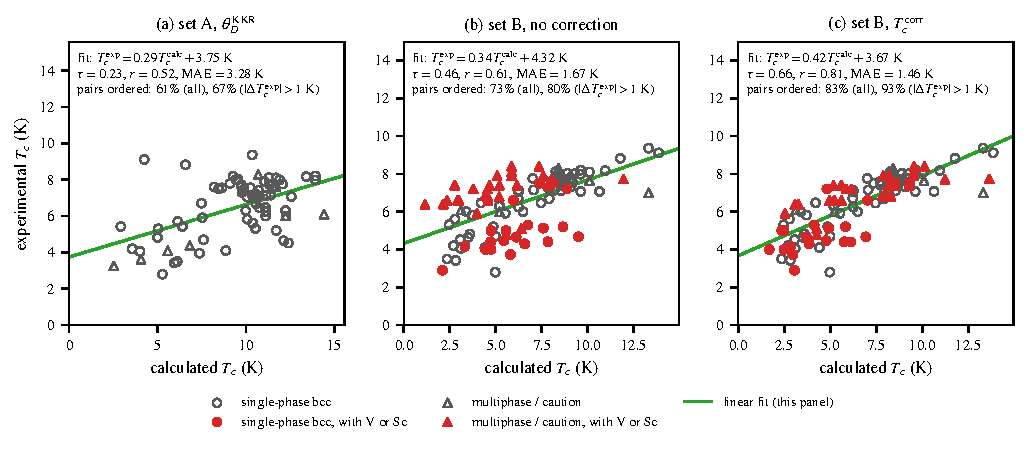
\includegraphics[width=\textwidth]{figS_validation_variants}
  \caption{As Fig.~1 of the main text, for (a) set~A with the Debye temperature
  $\theta_D^{\rm KKR}$ from the KKR-CPA elastic constants (Sec.~\ref{sec:debye}), (b) set~B
  without the correction of Sec.~III.B of the main text and (c) set~B with it. Filled red
  symbols in (b) and (c): alloys containing V or Sc, the only ones affected by the correction
  (bcc Debye temperature for Sc, electron--paramagnon coupling for V).}
  \label{fig:variants}
\end{figure}

Figure~\ref{fig:variants} and Table~\ref{tab:metrics} compare the variants of the estimator on
the literature set. Without the correction of Sec.~III.B of the main text the 47
V- or Sc-containing entries (18 with V, 30 with Sc) are essentially uncorrelated with
experiment ($\tau = 0.16$, 58\% of the pairs ordered); the V-rich alloys are overestimated and
the Sc-rich ones underestimated. The correction, which lowers the Debye temperature of Sc and
adds the electron--paramagnon coupling of V, brings this subset to $\tau = 0.64$
(82\% / 89\%) and the whole set~B to the level of set~A. The two parameters of the correction
were fitted on the same literature entries, so the set-B metrics are not an independent
test; the set-A metrics are (no parameter other than the global $\mu^*$).

\begin{figure}
  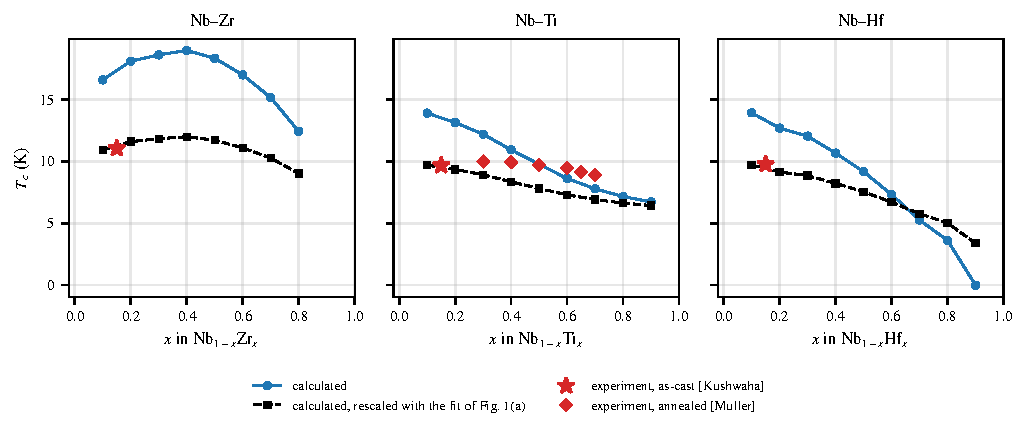
\includegraphics[width=\textwidth]{figS_binaries}
  \caption{Calculated \Tc\ along the Nb--Zr, Nb--Ti and Nb--Hf lines ($\mu^* = 0.1$,
  $\theta_D^{\rm mix}$): as calculated (circles) and rescaled with the linear fit of
  Fig.~1(a) of the main text, $T_c = 0.45\,T_c^{\rm calc} + 3.38$~K (squares). Stars:
  measured \Tc\ of as-cast Nb$_{0.85}X_{0.15}$~\cite{Kushwaha2025}; diamonds: resistive \Tc\ of
  recrystallised bcc Nb--Ti alloys~\cite{Muller1989}.}
  \label{fig:binaries}
\end{figure}

\emph{Binary alloys.} Figure~\ref{fig:binaries} shows the calculated \Tc\ along the binary
lines Nb--Zr, Nb--Ti and Nb--Hf. The linear fit of Fig.~1(a) of the main text was obtained on
multicomponent alloys only; applied to the binaries it gives 10.9--12.0~K for
Nb$_{1-x}$Zr$_x$ with $x = 0.1$--0.4, and 9.7 and 9.4~K (Ti), 9.7 and 9.2~K (Hf) at
$x = 0.1$ and 0.2, to be compared with the measured 11.06, 9.68 and 9.78~K of the as-cast
Nb$_{0.85}X_{0.15}$ alloys~\cite{Kushwaha2025}. Along the Nb--Ti line a set of recrystallised bcc
alloys is available~\cite{Muller1989}: the measured \Tc\ stays close to 10~K up to
$x_{\rm Ti} = 0.5$ (10.00, 9.94 and 9.71~K at $x_{\rm Ti} = 0.3$, 0.4 and 0.5) and falls to
8.91~K at $x_{\rm Ti} = 0.7$, whereas the calculated \Tc\ decreases steadily from the Nb-rich
end (12.2, 10.9, 9.8 and 7.8~K at $x_{\rm Ti} = 0.3$, 0.4, 0.5 and 0.7; 8.9, 8.4, 7.8 and
6.9~K after rescaling). The calculation thus places the Ti-rich alloys 1--2~K too low
relative to the Nb-rich ones. For the search this error is on the safe side with respect to
Nb--Zr, whose measured \Tc\ is higher than that of any Nb--Ti alloy.

\begin{table}
\caption{Validation metrics on the literature set. $n$: number of entries; $\tau$: Kendall
rank correlation; $r$: Pearson correlation; MAE, bias: mean absolute and mean signed error
(calculated $-$ measured) in K; pairs: fraction of alloy pairs whose experimental order is
reproduced, for all pairs and for pairs differing by more than 1~K.}
\label{tab:metrics}
\begin{ruledtabular}
\begin{tabular}{lrcccccc}
subset / estimator & $n$ & $\tau$ & $r$ & MAE & bias & pairs (all) & pairs ($>1$~K) \\
\hline
set A, $\mu^*=0.1$, $\theta_D^{\rm mix}$ & 74 & 0.66 & 0.84 & 1.40 & $+0.33$ & 0.83 & 0.94 \\
set A, single-phase only & 65 & 0.69 & 0.87 & 1.37 & $+0.31$ & 0.85 & 0.95 \\
set A, $\mu^*=0.2$ & 74 & 0.65 & 0.81 & 4.34 & $-4.34$ & 0.82 & 0.94 \\
set A, $\theta_D^{\rm KKR}$ & 74 & 0.23 & 0.52 & 3.28 & $+2.98$ & 0.61 & 0.67 \\
set B, no correction & 112 & 0.46 & 0.61 & 1.67 & $0.00$ & 0.73 & 0.80 \\
set B, $T_c^{\rm corr}$ & 112 & 0.66 & 0.81 & 1.46 & $+0.19$ & 0.83 & 0.93 \\
set B, single-phase only, $T_c^{\rm corr}$ & 80 & 0.68 & 0.87 & 1.31 & $+0.20$ & 0.84 & 0.94 \\
set B, entries with V or Sc, no correction & 47 & 0.16 & 0.16 & 2.03 & $-0.59$ & 0.58 & 0.52 \\
set B, entries with V or Sc, $T_c^{\rm corr}$ & 47 & 0.64 & 0.75 & 1.54 & $-0.13$ & 0.82 & 0.89 \\
A $\cup$ B, $T_c^{\rm corr}$ & 121 & 0.65 & 0.81 & 1.45 & $+0.15$ & 0.82 & 0.92 \\
\end{tabular}
\end{ruledtabular}
\end{table}

\clearpage
\section{Initial datasets}
\label{sec:init}

The composition of the initial datasets is given in Table~\ref{tab:init}. The interior
points are distributed as $\mathrm{Dirichlet}(1,\dots,1)$ over the ten elements, i.e.\
uniformly on the simplex; the face points have exactly $k$ non-zero elements. Counting only
elements above the 5\% threshold used by the optimiser, the interior points are mostly
five- to eight-component alloys, and the face points supply the binaries, ternaries and
quaternaries. The best points of the initial sets that satisfy the constraints of the
optimiser (no element above 70\%) are Nb$_{\sim 60}$Zr$_{\sim 40}$ face points with
18.8~K (set~A) and 18.7~K (set~B). A third dataset of 997 interior points only (no face points) was used
for the test of Sec.~\ref{sec:robust}.

\begin{table}
\caption{Initial datasets. Number of compositions with exactly $m$ non-zero elements (the
face points, $m=2,\dots,9$, and the interior points, $m=10$), and number with $m$ elements
above 5\%.}
\label{tab:init}
\begin{ruledtabular}
\begin{tabular}{lrrrrrrrrrrr}
 & total & $m=2$ & 3 & 4 & 5 & 6 & 7 & 8 & 9 & 10 \\
\hline
set A, non-zero elements & 1795 & 99 & 100 & 99 & 100 & 100 & 100 & 100 & 100 & 997 \\
set A, all elements above 5\% & 1795 & 99 & 111 & 146 & 283 & 417 & 376 & 232 & 128 & 3 \\
set B, non-zero elements & 1800 & 100 & 100 & 100 & 100 & 100 & 100 & 100 & 100 & 1000 \\
set B, all elements above 5\% & 1800 & 100 & 110 & 165 & 270 & 410 & 382 & 238 & 125 & 0 \\
\end{tabular}
\end{ruledtabular}
\end{table}

\clearpage
\section{Robustness of the optimisation}
\label{sec:robust}

\begin{figure}
  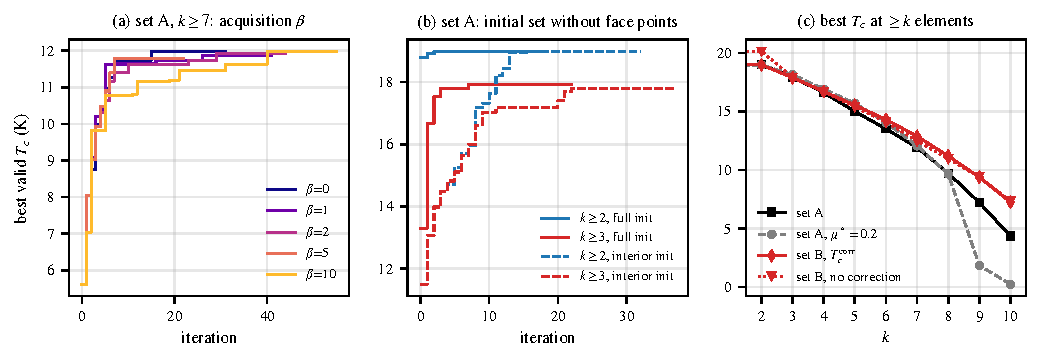
\includegraphics[width=\textwidth]{figS_robustness}
  \caption{(a) Best valid \Tc\ versus iteration for five runs of set~A with $k \geq 7$ that
  differ only in the weight $\beta$ of the acquisition score. (b) Runs with
  $k \geq 2$ and $k \geq 3$ started from the full initial set (solid) and from the interior
  points only (dashed). (c) Best \Tc\ at $\geq k$ elements: set~A; set~A with $\mu^* = 0.2$
  (runs for $k = 2$--8); set~B with and without the correction of Sec.~III.B of the main
  text.}
  \label{fig:robust}
\end{figure}

\begin{figure}
  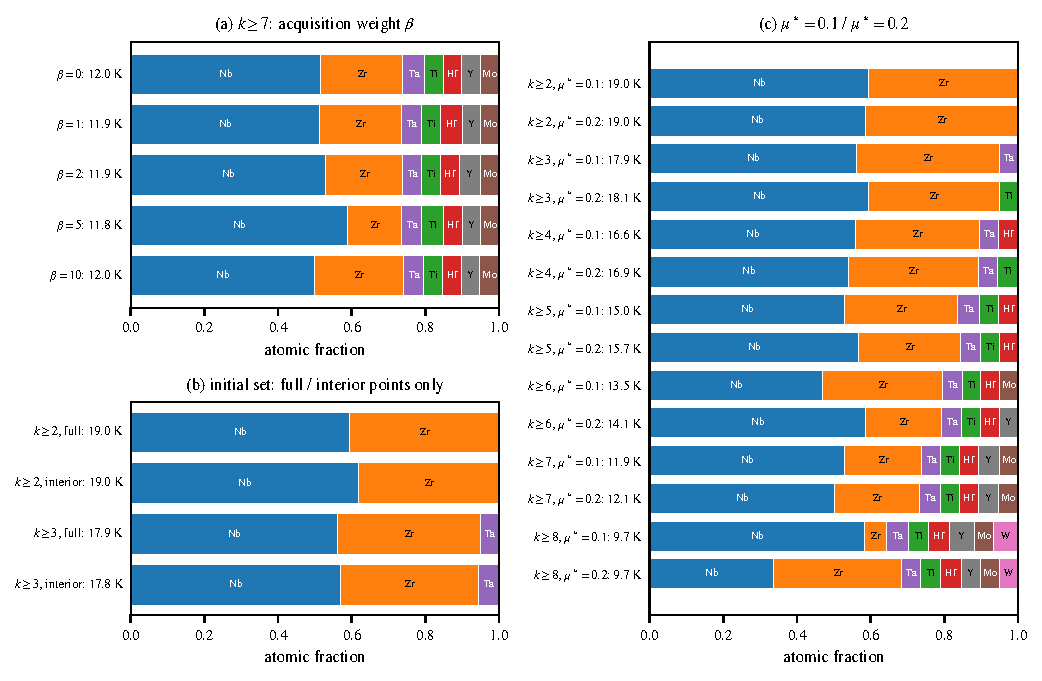
\includegraphics[width=\textwidth]{figS_robust_champions}
  \caption{Champion compositions and their \Tc\ in the test runs of set~A: (a) runs with
  $k \geq 7$ and different $\beta$; (b) runs with $k \geq 2$ and $k \geq 3$ started from the
  full initial set and from the interior points only; (c) runs with $\mu^* = 0.1$ (main text)
  and with $\mu^* = 0.2$ for $k = 2, \dots, 8$.}
  \label{fig:robust_champions}
\end{figure}

\emph{Acquisition weight.} Five runs of set~A with $k \geq 7$ and $\beta = 0, 1, 2, 5, 10$
end at 11.98, 11.88, 11.92, 11.79 and 11.98~K with champions of the same family,
Nb$_{50-59}$Zr$_{15-24}$ + Ta, Hf, Ti, Mo, Y at 5--6\% (Figs.~\ref{fig:robust}(a) and
\ref{fig:robust_champions}(a)).

\emph{Initial set without face points.} The optimum of a run with small $k$ lies on a
low-dimensional face of the simplex, far from the interior points, which all contain ten
elements. The runs with $k \geq 2$ and $k \geq 3$ are therefore the ones for which the
presence of face points in the initial set should matter most, and we repeated these two
runs starting from the 997 interior points only. Even then the optimiser moves to the edge of
the simplex by itself, within the constraint on the minimum number of elements, and arrives
at the same compositions: 18.98~K (Nb$_{62}$Zr$_{38}$) and 17.79~K
(Nb$_{57}$Zr$_{37}$Ta$_6$), against 18.99~K (Nb$_{59}$Zr$_{41}$) and 17.92~K
(Nb$_{56}$Zr$_{39}$Ta$_5$) from the full set (Figs.~\ref{fig:robust}(b) and
\ref{fig:robust_champions}(b)). The only difference is the length of the search: the
champion is found after 17 and 22 iterations instead of 3 and 7. The face points of the
initial set thus shorten the search but do not determine its result.

\emph{Runs with $\mu^* = 0.2$.} A separate series of set-A runs for $k = 2, \dots, 8$ used
$\mu^* = 0.2$ and a cap of 75\% on a single element. In these runs the McMillan--Hopfield
parameter was obtained differently (matrix elements from a radial integration with an inner
cutoff, and the site-projected instead of the total density of states in the prefactor),
which gives larger coupling constants ($\lambda = 1.54$ instead of 1.14 for Nb--Zr), so that
with $\mu^* = 0.2$ the absolute scale of \Tc\ again matches the literature set; the two
series therefore differ in the pair $(\lambda, \mu^*)$ and not in $\mu^*$ alone. Their best
\Tc\ at $\geq k$ elements, 18.96, 18.14, 16.90, 15.69, 14.06, 12.06 and 9.66~K, agree with
those of the main text within 0.2--0.7~K (Fig.~\ref{fig:robust}(c)), and the champions belong
to the same Nb--Zr family with the same elements at the 5\% floor
(Fig.~\ref{fig:robust_champions}(c)); the differences are the choice between Ta and Ti as
the third element for $k = 3$ and 4, Y instead of Mo for $k = 6$, and a Zr-rich instead of
a Nb-rich alloy for $k = 8$.

\emph{Set B without the correction.} With the uncorrected $T_c$ as target the set-B champions
are 20.14~K (V$_{68}$Ti$_{32}$, the overestimated Ti--V system of Sec.~III.B), 17.90, 16.72,
15.39, 14.08, 12.49, 10.95, 9.41 and 7.34~K for $k = 2, \dots, 10$. Apart from the binary they
lie within 0.6~K of the set-A front up to $k = 7$ and 1.2--3.0~K above it for $k = 8$--10,
with V instead of Sc as the first 3$d$ element at the floor (Fig.~\ref{fig:robust}(c)).
Along the Ti--V line the uncorrected estimator gives 17.8--20.6~K for $x_{\rm Ti} =
0.1$--0.5, against measured values below 8~K~\cite{Matin2014}.

\clearpage
\section{Physics of the optimised compositions}
\label{sec:physics}

\begin{figure}
  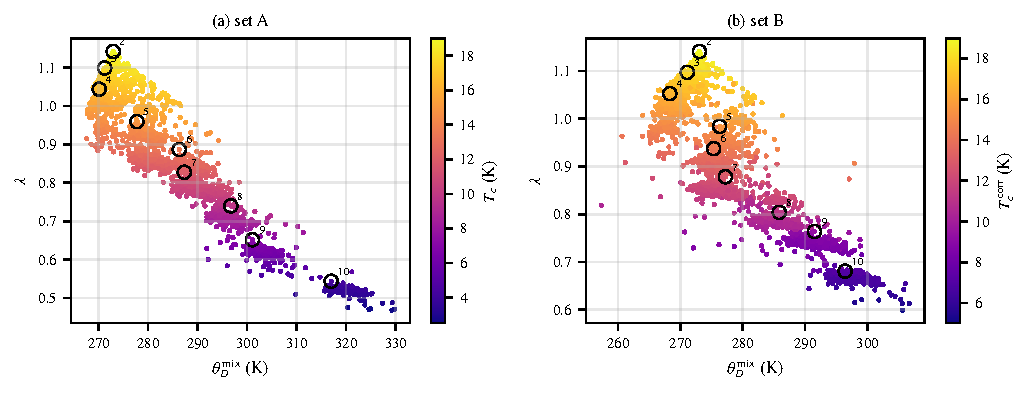
\includegraphics[width=\textwidth]{figS_lambda_theta}
  \caption{Electron--phonon coupling constant versus mixture Debye temperature for all
  compositions proposed by the optimiser in (a) set~A and (b) set~B, coloured by the
  calculated \Tc. Circles: champions of the runs with $k = 2, \dots, 10$.}
  \label{fig:lamtheta}
\end{figure}

Figure~\ref{fig:lamtheta} shows $\lambda$ against $\theta_D^{\rm mix}$ for all compositions
proposed by the optimiser. The points fall on a narrow band: adding elements to Nb--Zr
lowers $\lambda$ and raises $\theta_D^{\rm mix}$ at the same time, and the colour scale shows
that \Tc\ follows $\lambda$ (correlation 0.998 in set~A, 0.98 in set~B) while the increase of
$\theta_D$ only slightly offsets the loss. The champions of successive $k$ move along the band
from $(\lambda, \theta_D) = (1.14, 273~{\rm K})$ to $(0.55, 317~{\rm K})$ in set~A.

\clearpage
\section{Structural and thermodynamic data}
\label{sec:td}

The bcc/fcc/hcp comparison of Table~I of the main text uses, for each structure, seven
lattice constants fitted with a Birch--Murnaghan equation of state (hcp additionally at
five $c/a$ ratios), with the same KKR-CPA settings as the lattice stage of the pipeline.
The pure-element references were computed in the same way. The calculated bcc--hcp energy
differences of the elements (meV/atom; positive = hcp lower): Ti 38, Zr 5, Hf 132, Y 59,
Sc 50, Ru 518, Re 162; Nb $-417$, Ta $-462$, V $-341$, Mo $-543$, W $-712$. These reproduce the
ground states but, as is usual for muffin-tin KKR energies, overestimate the magnitude of
the bcc--hcp separation of the group-5 and group-6 metals; the alloy values in Table~I of
the main text should therefore be read as upper bounds on the bcc preference, which does not
affect the conclusion.

For pure W and Re the energy window of 0.6~Ry used throughout does not enclose the bottom of
the valence band: with this window the W equation of state has its minimum at 6.26~bohr
(experiment 5.98~bohr) and the Re one is unphysical (bulk modulus of order $10^4$~GPa, bcc
ground state). The total energy of bcc W at fixed lattice constant changes by 62~mRy between
windows of 0.6 and 1.0~Ry, but by less than 1~mRy for all windows of 0.75~Ry and wider; for Re
the energies obtained with 0.9, 1.0 and 1.3~Ry agree within 0.3~mRy. The references of W and Re
were therefore computed with a 1.0~Ry window ($a_0$ = 6.01~bohr for bcc W, hcp ground state of
Re). Converged energies do not depend on the window: for Ti, Nb, Zr, Ta, Mo and Y the bcc
energies obtained with 0.6 and 1.0~Ry differ by 1--5~meV/atom, and for the two Re-containing
champions (at $a_0$, about 5\% each of W and Re) the energies obtained with 0.6 and 0.7~Ry
differ by less than 0.1~mRy, so the alloys and the other elements were kept at 0.6~Ry. A single
wider window for all calculations is not possible: for Hf the SCF iteration does not converge
for windows of 0.75~Ry and wider, at which the contour reaches the Hf 4$f$ level. The bcc
reference energies of the other elements used for $\Delta H_{\rm bcc}$ agree with the present
calculations within 2.3~meV/atom, except Ru (6~meV/atom).

\clearpage
\section{Choice of the Coulomb pseudopotential}
\label{sec:mustar}

The Coulomb pseudopotential is the only parameter of Eq.~(3) of the main text that is not
calculated. McMillan~\cite{McMillan1968} proposed $\mu^* = 0.13$ for the transition metals, and
values between 0.1 and 0.15 are the common choice when \Tc\ is estimated from a calculated
or measured $\lambda$~\cite{McMillan1968,AllenDynes1975,lit_Idczak_16175814,lit_Idczak_fnz7bzmw}.
Considerably larger values have been used when a calculated coupling constant had to be
reconciled with the measured \Tc: $\mu^* = 0.21$ for Nb and 0.30 for V with
linear-response Eliashberg functions~\cite{Savrasov1996}, 0.24 for
Nb$_3$Ge~\cite{Carbotte1990}, 0.20--0.25 and 0.215 for the Ta--Nb--Hf--Zr--Ti
high-entropy alloy with rigid-muffin-tin coupling
constants~\cite{Jaskiewicz2016,Jaskiewicz2019}, and 0.21 for
(NbTa)$_{0.67}$(MoHfW)$_{0.33}$~\cite{lit_Sobota_06184512}. In such cases $\mu^*$ acts as an
effective parameter that absorbs the error of $\lambda$ and of the phonon frequencies, and
its value is tied to the way $\lambda$ was obtained.

The same holds here. Figure~\ref{fig:mustar} shows the agreement between the calculated and
measured \Tc\ of the literature alloys (Table~\ref{tab:lit}) as a function of $\mu^*$, all
other ingredients being fixed. The absolute scale depends strongly on $\mu^*$: the median
ratio of calculated to measured \Tc\ falls from 1.56 at $\mu^* = 0.05$ to 1.05 at 0.10, 0.77
at 0.13, 0.30 at 0.20 and 0.02 at 0.30 (set~A), and the mean absolute error has a sharp
minimum of 1.4~K at $\mu^* = 0.10$--0.11 in both sets (1.7--1.8~K at 0.13, 4.3--4.4~K at
0.20). The ordering of the alloys, in contrast, hardly depends on $\mu^*$: Kendall's
$\tau$ changes from 0.67 to 0.62 between $\mu^* = 0.05$ and 0.30, and the fraction of
correctly ordered pairs that differ by more than 1~K stays at 93--94\% in set~A and at
93\% in set~B. The value
$\mu^* = 0.1$ used throughout is therefore a calibration of the absolute scale of our
estimator, with the Lloyd normalisation of $\eta$ and $\theta_D^{\rm mix}$, and not a
statement about the screened Coulomb interaction in these alloys; with a different
evaluation of $\eta$ the calibrated value is different (0.2 for the alternative evaluation of
Sec.~\ref{sec:robust}).

\begin{figure}
  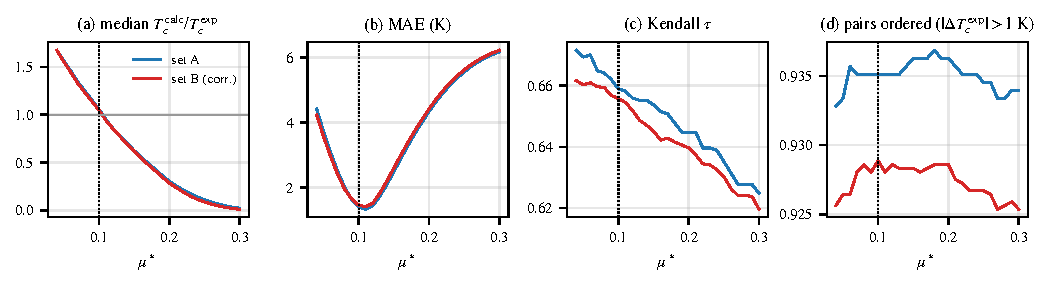
\includegraphics[width=\textwidth]{figS_mustar_baseline}
  \caption{Agreement between calculated and measured \Tc\ of the literature alloys as a
  function of $\mu^*$ for set~A (74 entries, Eq.~(3) of the main text) and set~B (112
  entries, corrected estimator): (a) median ratio, (b) mean absolute error, (c) Kendall's
  $\tau$, (d) fraction of correctly ordered pairs among those with measured \Tc\ differing
  by more than 1~K. The dotted line marks $\mu^* = 0.1$.}
  \label{fig:mustar}
\end{figure}

\clearpage
\section{Optimised compositions at other values of $\mu^*$}
\label{sec:mustar_champions}

Table~\ref{tab:mustar} and Fig.~\ref{fig:mustar_champions} give \Tc\ of the champion
compositions of the main text, re-evaluated with $\mu^* = 0.05$, 0.2 and 0.3 from the same
$\lambda$ and $\theta_D^{\rm mix}$ (the compositions were optimised with $\mu^* = 0.1$ and
are not re-optimised here). The absolute values scale as expected from
Sec.~\ref{sec:mustar}, from 22.9~K to 5.5~K for the Nb--Zr binary, but the monotonic
decrease of \Tc\ with the number of constituents is the same for every $\mu^*$, because
$\lambda$ decreases along the series while $\theta_D^{\rm mix}$ changes little. The loss
between $k = 2$ and $k = 10$ is 15.3, 14.6, 11.0 and 5.5~K in set~A and 12.1, 11.7, 9.5 and
5.3~K in set~B for $\mu^* = 0.05$, 0.1, 0.2 and 0.3, respectively. An independent optimisation
with a different estimator calibrated to $\mu^* = 0.2$ leads to the same compositions
(Sec.~\ref{sec:robust}).

\begin{figure}
  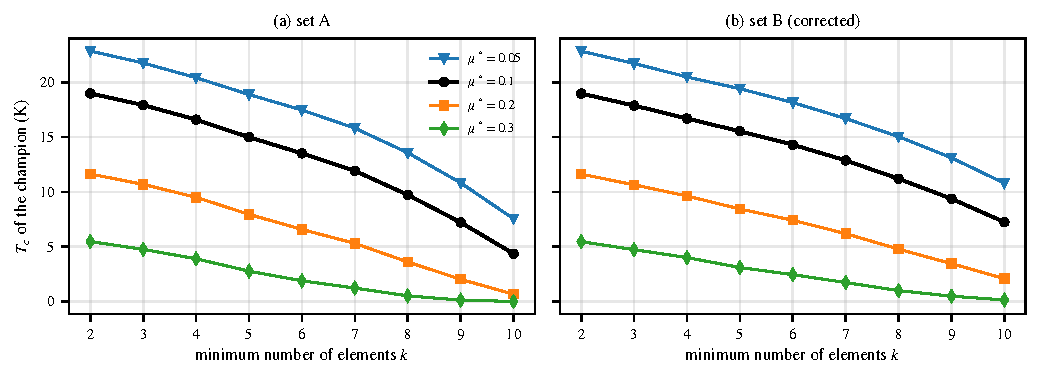
\includegraphics[width=\textwidth]{figS_mustar_champions}
  \caption{\Tc\ of the champion compositions of (a) set~A and (b) set~B (corrected
  estimator) for four values of $\mu^*$. The compositions are those found with
  $\mu^* = 0.1$ (thick line).}
  \label{fig:mustar_champions}
\end{figure}

\begin{table}
\caption{Champion compositions of the runs with at least $k$ elements: coupling constant,
Debye temperature (for set~B the corrected values of Sec.~III.B of the main text) and
\Tc\ (K) for four values of $\mu^*$.}
\label{tab:mustar}
\begin{ruledtabular}
\begin{tabular}{cccccccc}
set & $k$ & $\lambda$ & $\theta_D^{\rm mix}$ (K) & $\mu^*=0.05$ & 0.1 & 0.2 & 0.3 \\
\hline
A & 2 & 1.14 & 273 & 22.9 & 19.0 & 11.6 & 5.5 \\
A & 3 & 1.10 & 271 & 21.8 & 17.9 & 10.7 & 4.8 \\
A & 4 & 1.04 & 270 & 20.4 & 16.6 & 9.5 & 3.9 \\
A & 5 & 0.96 & 278 & 18.9 & 15.0 & 7.9 & 2.8 \\
A & 6 & 0.89 & 286 & 17.5 & 13.5 & 6.6 & 1.9 \\
A & 7 & 0.83 & 287 & 15.8 & 11.9 & 5.3 & 1.2 \\
A & 8 & 0.74 & 297 & 13.6 & 9.7 & 3.6 & 0.5 \\
A & 9 & 0.65 & 301 & 10.8 & 7.2 & 2.0 & 0.1 \\
A & 10 & 0.54 & 317 & 7.5 & 4.4 & 0.7 & 0.0 \\
\hline
B & 2 & 1.14 & 273 & 22.8 & 19.0 & 11.6 & 5.5 \\
B & 3 & 1.10 & 271 & 21.7 & 17.9 & 10.7 & 4.7 \\
B & 4 & 1.05 & 268 & 20.5 & 16.7 & 9.6 & 4.0 \\
B & 5 & 0.98 & 276 & 19.4 & 15.5 & 8.4 & 3.1 \\
B & 6 & 0.94 & 275 & 18.2 & 14.3 & 7.4 & 2.4 \\
B & 7 & 0.88 & 277 & 16.7 & 12.9 & 6.2 & 1.7 \\
B & 8 & 0.80 & 286 & 15.0 & 11.2 & 4.8 & 1.0 \\
B & 9 & 0.76 & 292 & 13.1 & 9.4 & 3.5 & 0.5 \\
B & 10 & 0.68 & 296 & 10.8 & 7.2 & 2.1 & 0.1 \\

\end{tabular}
\end{ruledtabular}
\end{table}

\bibliography{refs}

\end{document}
